\documentclass[journal,10pt,onecolumn,compsoc,letterpaper,draftclsnofoot,table,xcdraw]{IEEEtran} \usepackage[margin=0.75in]{geometry}
\usepackage{pdfpages}
\usepackage{minted}
\usepackage{graphicx,float} 
\usepackage{listings}
\usepackage{verbatim}
\usepackage{url}
\usepackage{nameref}
\usepackage{setspace} \singlespacing
\graphicspath{/graphics} \setlength{\parskip}{\baselineskip} \setlength\parindent{24pt}
\usepackage[english]{babel}
\usepackage{fullpage}
\usepackage{hyperref}
\hypersetup{
    colorlinks,
    citecolor=black,
    filecolor=black,
    linkcolor=black,
    urlcolor=black
}
\title{Final Project: Processes, I/O and Memory Management}
\author{Behnam Saeedi\\ CS444: Operating systems II}
\date{\today}
\begin{document}
\maketitle
\begin{centering}
Spring 2017
\begin{abstract}
\noindent This document is the final project for CS444 Operating systems II class for the Spring term of 2017. The first operating system with the commercial name of Windows was released in 1990 at version 3.0. Followed by that in 1991 the first version of Linux operating system was released at version 0.01-0.1. Two years after that in 1993 the first distribution of FreeBSD was released to the public. Each one of these operating systems have a specific target audience and excel at performing certain operations. Many generations of these Operating systems have been released and they have gone through many changes since the first distributions of these kernels. They provide series of supports and services to the users and some are capable of performing certain tasks better than others. There are 3 topics presented in this document. These topics are Processes, I/O and Memory Management. This document will cover these three topics in 3 Operating systems. These operating systems are Linux, Windows and FreeBSD. After the material with regards to each one of the three topics a comparison is provided in order to demonstrate some of the differences between these kernels and compare them based on performance and approach. The first subsection of each kernel describes the implementation of processes, threads and CPU schedulers that are used in Linux, Windows and FreeBSD kernels. The second subsection of each kernel analyzes them based on the data structures, schedulers, algorithms, cryptography and I/O scheduling. The third and last subsection of each kernel section covers some of the details about how the memory management features implemented, what are some of their features and how do they stack up against Linux's implementation of those features. These information has been gathered by looking into a wide variety of resources which are listed in the references section of this document.
\end{abstract}
\end{centering}
%--------------------------------------------------------------
\newpage
\tableofcontents
\newpage 
%--------------------------------------------------------------
\section{Introduction}
\noindent An operating system has a set of responsibilities in order to allow users to be able to use their hardware. Among these requirements are important elements such as concurrent operations and processes, Input and output of file and memory management, interrupt handling and filesystem. Each one of these requirements are important for the operating system's performance. Linux, Windows and FreeBSD provide different solutions in order to satisfy these requirements. Each operating system provides its solution based on their target user and performance needs of kernel. Following sections will cover Linux Processes, I/O and Memory management in order to develop a control for comparison. Next section covers the same concepts from a windows perspective. It will cover the design and implementation of each item and provides a comparison of their approach with Linux. Finally, This document looks into the Processes, I/O and memory management of the FreeBSD operating system. Similar to windows section, a comparison will be provided between Linux and FreeBSD.
%--------------------------------------------------------------
\section{Linux}
\noindent The first Operating system that this document covers is the Linux Operating system. Linux 0.01-0.1 was developed in 1991. It lacked many features that we take for granted for our modern operating systems, include a graphical user interface. in the past 26 years, Linux has come a long way and the newest version of Linux is 16.04 LTS. This section covers the Processes, I/O and memory management features of Linux operating system. 
\subsection{Process}
\subsubsection{Process}
\noindent In Linux processes are instances of running programs. In Linux the first process that is created with ID 1 is the init process. The processes could be viewed by two commands:
\begin{minted}{bash}
$ top
# and
$ ps
\end{minted}

\begin{figure}[ht]
\centering
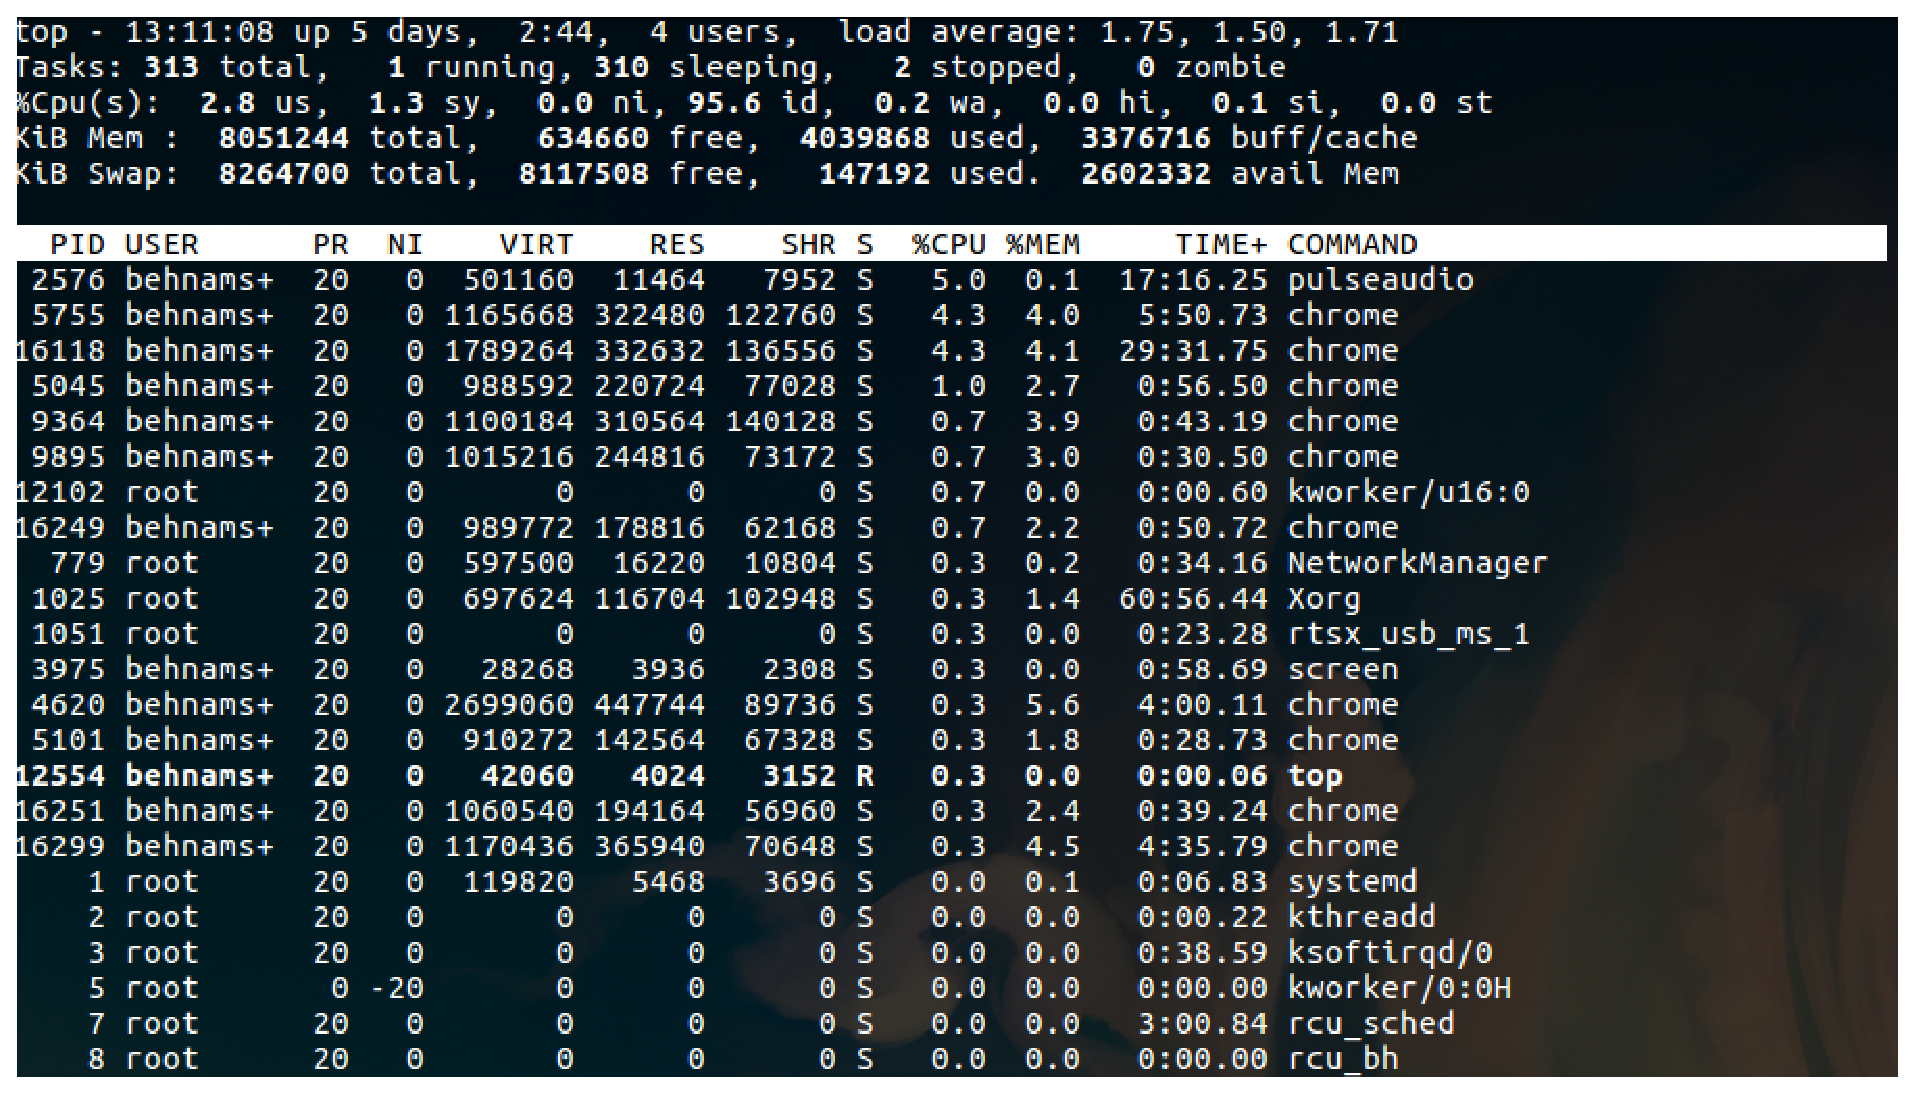
\includegraphics[width=150mm]{graphics/Top-view} \\
\caption{The view of "top" command in Linux shell}
\end{figure}

\begin{figure}[ht]
\centering
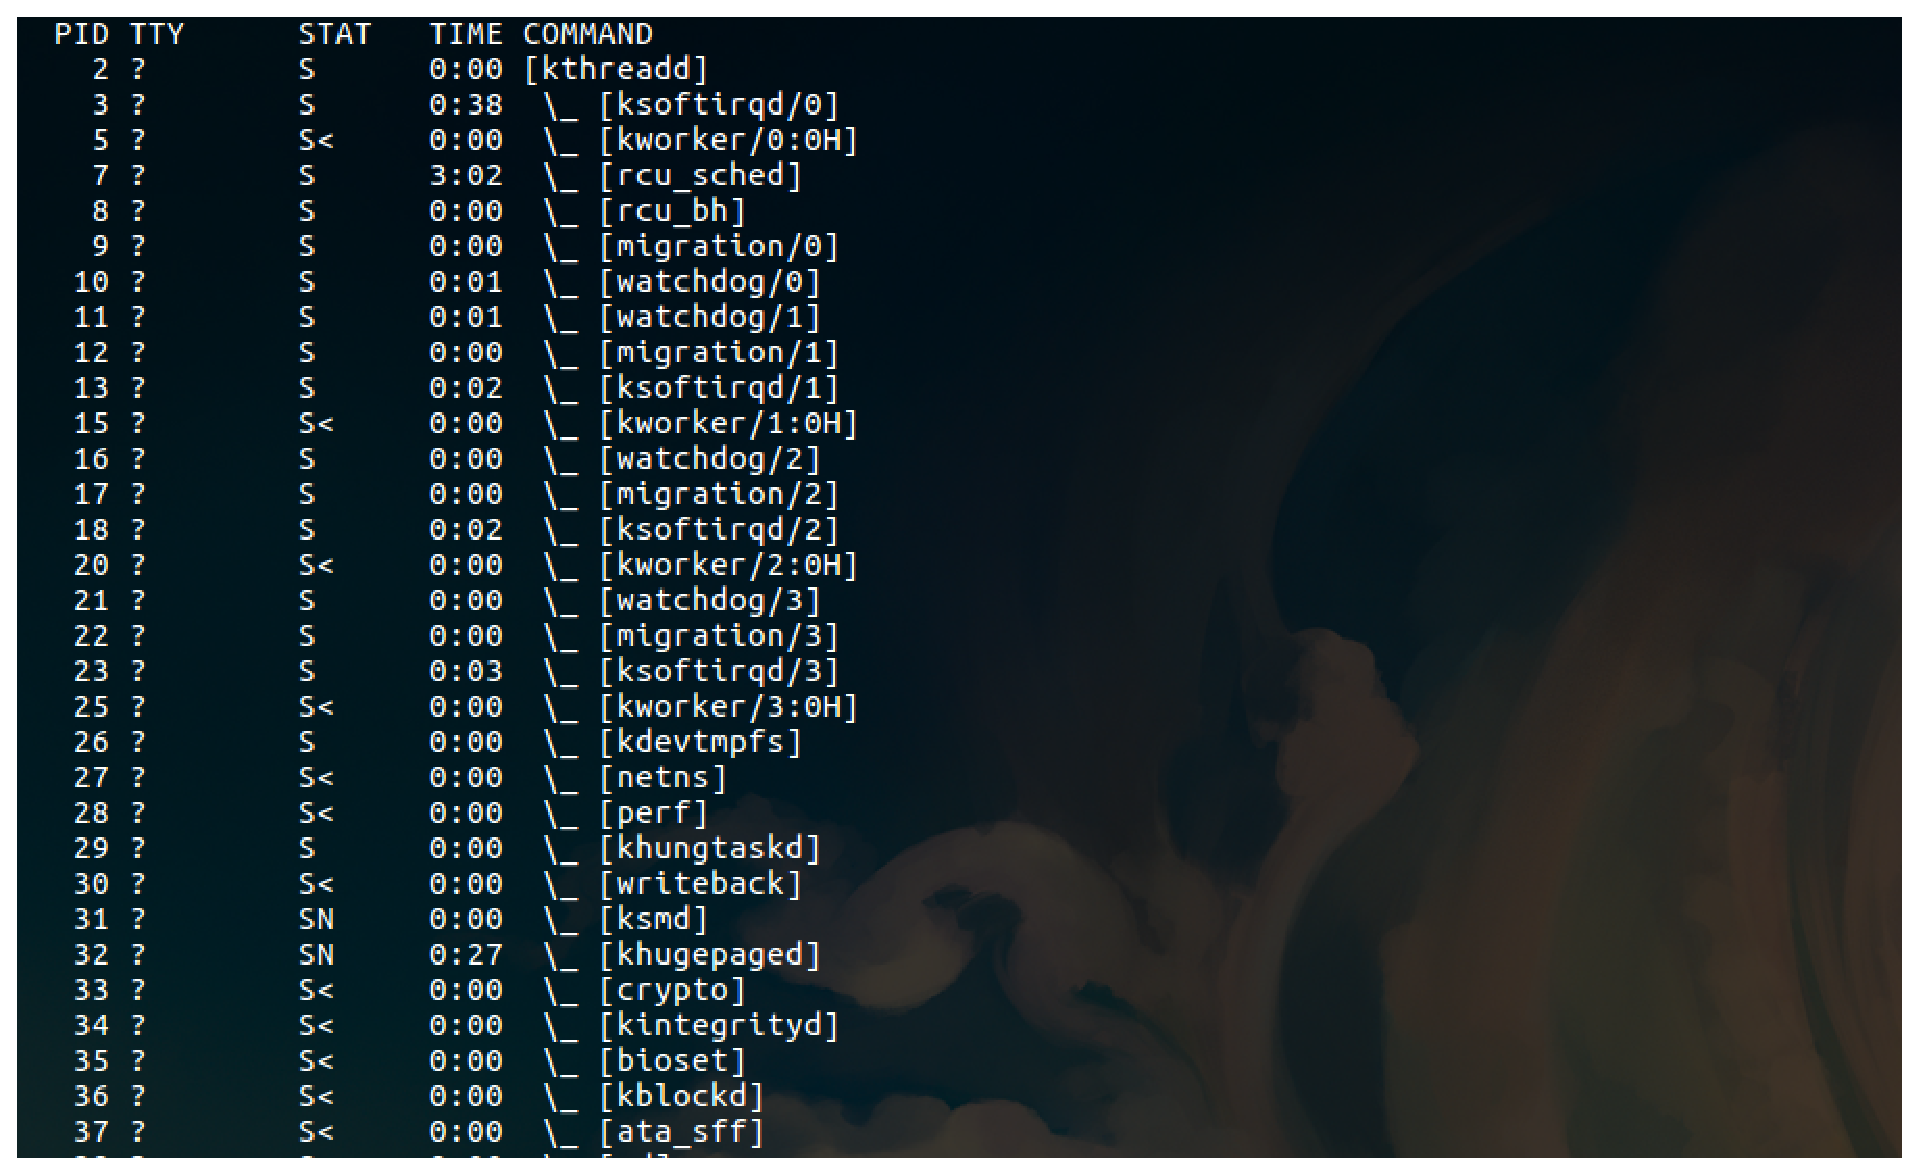
\includegraphics[width=150mm]{graphics/ps} \\
\caption{The view of "ps fax" command in shell}
\end{figure}

\noindent These two commands show a list of processes that are happening on the operating system. figures 1,2. top is a live view and ps is a static view of current processes. The init process could be found and viewed by the following command:
\begin{minted}{bash}
$ ps fax | grep [i]nit
    1 ?        Ss     0:06 /sbin/init splash
\end{minted}
\noindent Each process in Linux could be in one of the following states:
\begin{itemize}
\item \textbf{Running:} Task is being processed or is about to be assigned to CPU for process.
\item \textbf{Waiting:} interruptible and un-interruptible process waiting for resources to be assigned.
\item \textbf{Stopped:} The process has been stopped by a signal. The process is in a halt.
\item \textbf{Zombie :} This is a terminated process that is still consuming resources.
\end{itemize}

\noindent In Linux each process has an identifier and a task vectors. in order to see this feature better, Linux provides the "pstree" command:
\begin{minted}{bash}
$ pstree
systemd─┬─ModemManager─┬─{gdbus}
        │              └─{gmain}
        ├─NetworkManager─┬─dhclient
        │                ├─dnsmasq
        │                ├─{gdbus}
        │                └─{gmain}
        ├─Xvfb─┬─{llvmpipe-0}
        │      ├─{llvmpipe-1}
        │      ├─{llvmpipe-2}
        │      └─{llvmpipe-3}
        ├─accounts-daemon─┬─{gdbus}
        │                 └─{gmain}
        ├─acpid
        ├─agetty
        ├─at-spi-bus-laun─┬─dbus-daemon
        │                 ├─{dconf worker}
        │                 ├─{gdbus}
        │                 └─{gmain}
        ├─at-spi2-registr─┬─{gdbus}
        │                 └─{gmain}
        ├─avahi-daemon───avahi-daemon
        ├─bluetoothd
#			.
#			.
#			.
\end{minted}
\noindent Task vector is an array of pointers in a data structure sense that points to ever task struct data structure in the system. Furthermore, Unix introduced a system known as IPC or Inter-Process Communication. This allows different processes to communicate with one another.
\subsubsection{Thread}
\noindent From the kernel's perspective there is no distinction between threads and processes. Threads are series of processes that get access to the same memory space. From a CPU and scheduling perspective each thread gets its own time slot. We can trace and see each of these threads that are related to a process. Running the following code reveals an interesting fact about the Linux processes:
\begin{minted}{bash}
$ Htop
# or
$ top -H
# or
$ ps -T -p 1
\end{minted}
\noindent init actually does not lunch any threads meaning that non of its children and the init itself would have access to the memory space of the child processes. Using the following command we can see the threads of each process:
\begin{minted}{bash}
$ ps -T -p $(ps efax | grep [m]y-app | awk '{print $1}')
# replace my-app with name of a program such as mysqld -> [m]ysqld
$ ps -T -p $(ps efax | grep [m]ysqld | awk '{print $1}')

  PID  SPID TTY          TIME CMD
 8302  8302 ?        00:00:00 mysqld
 8302  8307 ?        00:00:00 mysqld
 8302  8308 ?        00:00:03 mysqld
 8302  8309 ?        00:00:04 mysqld
 8302  8310 ?        00:00:03 mysqld
 8302  8311 ?        00:00:03 mysqld
 8302  8312 ?        00:00:03 mysqld
 8302  8313 ?        00:00:03 mysqld
 8302  8314 ?        00:00:03 mysqld
 8302  8315 ?        00:00:03 mysqld
 8302  8316 ?        00:00:03 mysqld
 8302  8317 ?        00:00:03 mysqld
 8302  8318 ?        00:00:03 mysqld
 8302  8320 ?        00:00:03 mysqld
 8302  8321 ?        00:00:05 mysqld
 8302  8322 ?        00:00:00 mysqld
 8302  8323 ?        00:00:04 mysqld
 8302  8324 ?        00:00:00 mysqld
 8302  8325 ?        00:00:00 mysqld
 8302  8326 ?        00:00:00 mysqld
 8302  8327 ?        00:00:00 mysqld
 8302  8328 ?        00:00:00 mysqld
 8302  8329 ?        00:00:00 mysqld
 8302  8330 ?        00:00:00 mysqld
 8302  8331 ?        00:00:00 mysqld
 8302  8332 ?        00:00:00 mysqld
 8302  8333 ?        00:00:00 mysqld
 8302  8336 ?        00:00:00 mysqld

\end{minted}
\noindent All of these threads use the same address space as the mysqld process that was displayed in ps. In implementation, thread is actually implemented as a process. We can imagine process as a memory space and threads as units of execution of the program. many programs have a single threads for the process. Kernel to has a 1-1 ratio between both of them, it treats threads as full processes that share the same memory space. Even we try to spawn a new thread we use the same command as spawning a new process and pass different arguments to indicate if we want our new thread to be independent process or not.
\subsubsection{CPU Scheduling}
\noindent Linux uses complex data structures in order to become very efficient in binding processes to the CPU. Each processor gets its own run queue and selects processes from that specific run queue. This creates an issue where one processor ends up idling while there are processes on other processor's queue. In order to avoid this, the queues get rebalanced periodically. Each process gets a bitmask in order to identify which processor it can be processed on. This mask could be reassigned but re-balancing will not override affinity. The processor follows the following algorithm: \cite{cscedu}[page 6]
\begin{itemize}
\item Highest priority queue with runnable processes is selected
\item First process on that queue is selected
\item Quantum size is calculated
\item Runs until its time runs out
\item its put on the expire queue
\item the process repeats
\end{itemize}
\noindent As of 2007-04-13 a new patch put the CFS or completely fair scheduler in Linux kernel. \cite{cfsmemo}. As this memo mentions, a complete rewrite of the Linux task scheduler goes into place after this patch and replaces the O(1) scheduler that was used before. This scheduler follows the following algorithm: \cite{cfshw}
\begin{itemize}
\item The left most node of the scheduling tree is sent for execution.
\item If completed, it is removed from the system and scheduling tree.
\item If reached maximum execution time, it is stopped (voluntarily or via interrupt) and reinserted into the scheduling tree and a new execution time is calculated
\item repeat
\end{itemize}

\subsection{I/O}
\noindent In this subsection we are going to have a closer look on the I/O aspect of three common operating systems. These Operating systems are Linux, Windows and FreeBSD. In the first section we will cover the Linux in order to hold it a control to compare the other two operating system s to it. In this section we will talk about data structures, I/O scheduling, Cryptography and implementations.
\subsubsection{Data Structure}
\noindent According to Linux documentation the Linux Kernel provides various versions of double linked list specifically purposed for I/O. Some examples of these data structures are doubly linked list, B+ tree, priority heap and many many more. \cite{1}. Everything that requires a data structure in Linux is dependent on these few models. The thing to consider is that the Linux actually does not create a data based structure. Instead it provides the pointers needed in order to link them. The developers can create their own structs and include this pointer structure into their data containers. This has an interesting and useful side effect. Due to this method of implementation user has the capability to generate a linked list where the type of the data elements does not need to match. This means a link containing and integer could be followed by a link that contains character.
\subsubsection{Algorithms}
\noindent There are many different scheduling algorithms. These algorithms include: 
\begin{itemize}
\item Random scheduling (RSS)
\item First In, First Out (FIFO), also known as First Come First Served (FCFS)
\item Last In, First Out (LIFO)
\item Shortest seek first, also known as Shortest Seek / Service Time First (SSTF)
\item Elevator algorithm, also known as SCAN (including its variants, C-SCAN, LOOK, and C-LOOK)
\item N-Step-SCAN SCAN of N records at a time
\item FSCAN, N-Step-SCAN where N equals queue size at start of the SCAN cycle
\item Completely Fair Queuing (CFQ) on Linux
\item Anticipatory scheduling
\item Noop scheduler
\item Deadline scheduler
\item mClock scheduler \cite{2}
\item Budget Fair Queuing (BFQ) scheduler \cite{3}
\item Kyber \cite{4}
\end{itemize}
\subsubsection{I/O scheduling}
\noindent Checking the Linux kernel files we can see that the algorithms which Linux supports are NOOP, deadline, and CFQ. In previous assignment we implemented the SSTF version for Linux. (it is good to note that there are 3rd party implementations of that available).
\subsubsection{Cryptography}
\noindent Linux provides one of the most extensive cryptographic APIs available. It supports a wide variety of algorithms available for memory. There is an extensive list of cypher alogrithms available: \cite{5}
\begin{itemize}
\item Symmetric ciphers
\item AEAD ciphers
\item Message digest, including keyed message digest
\item Random number generation
\item User space interface
\end{itemize}
\noindent These algorithms are used in order to create the following templates available to the users: \cite{6}
\begin{itemize}
\item aes: or The Advanced Encryption Standard is a symmetric block cypher
\item ecb(aes): or Electronic Codebook and block mode of operations
\item cmac(aes): or Cipher-based Message Authentication Code
\item ccm(aes): or  Counter with CBC-MAC
\item rfc4106(gcm(aes)): Galois/Counter Mode (GCM) in Advanced Encryption Standard
\item sha1: or Secure Hash Algorithm 1 which is crypto-hash function
\item hmac(sha1): or Keyed-hash message authentication code (HMAC) 
\end{itemize}
\noindent As mentioned, the Linux Kernel provides both synchronous and asynchronous operations depending on the users need.

\subsection{Memory Management}
\subsubsection{Memory Management}
\noindent Due to size limitations on the amount of memory available to a kernel it is extremely important to have a subsystem dedicated to organize and manage distribution and handling of memory. This task falls under Kernel's responsibilities under Kernel utilities known as Memory management tools. This section will be covering the basics of Linux Kernel's memory management tools in depth. Furthermore, it will proved a brief description of Pages, Services, Features and capabilities of Linux Kernel's memory management.
\subsubsection{Services}
\paragraph{VM} Linux provides the memory to processes at the same time through a concept known as virtual memory. This means every process has access to all of the memory at the same time giving it the illusion of a much larger memory than the actual physical RAM.\cite{2-1}
\paragraph{Address Space Protection}Linux Kernel Guarantees that each memory gets it own virtual address space. Each virtual address space is completely independent of others and is achieved through offsets in memory.\cite{2-1}
\paragraph{Memory Mapping} In Linux, files could be mapped directly to to a processes virtual address space. This process is known as memory mapping. This feature is one of the requirements for the memory management and is present in Linux, Windows and FreeBSD.\cite{2-1}
\subsubsection{Pages} Since the size of the virtual memory is significantly larger than the physical memory there is a need for a reliable way to address the memory. The process of assigning the virtual memory to the physical memory is known as paging. Pages are 4KB units of contiguous memory on the RAM and the basic unit of memory known by both Kernel and the CPU. This is regardless of the fact that both Kernel and CPU do have access to individual bits written on each page.\cite{2-2}. The operating system could fall into two dangerous scenarios: Data Collision and unused data. These two problems are the two extremes of the problems that can occur. memory collision happens when one physical memory is addressed by more than one virtual memory. The second issue occurs when a physical memory is not addressed by any virtual memory of running processes and is not being used efficiently.\cite{2-1}
\paragraph{Efficiency and Demand Paging} One way of preserving efficiency of the program is to avoid allocation of virtual memory while the process is not running. This is known as Demand Paging. Linux uses this method to take care of file load and maps it to the memory.\cite{2-1}
\subsubsection{Features}
\noindent Linux kernel provides a set of features that allow users to fully take advantage of the provided memory.
\paragraph{Cache} As discussed in the class, in order to have the programs run more efficiently, concept of caching is introduced. Task of this feature is to keep a copy of the data for future use with a faster access time than the storage drive. This process is known as caching and it can take place on several different levels.
\begin{itemize}
\item Buffer Cache: Block device driver's data buffers \label{BC}
\item Page Cache: Memory map speed boost (allowing faster file access)
\item Swap Cache: file data that is going to be kicked off of the memory. (dirty pages only)
\item Hardware Cache: Translation, look-aside buffers \cite{2-1}. CPU will not check the entire memory every time it needs access to data.\label{HWC}
\end{itemize}
\paragraph{Swapping} What if a process requires a memory and there are no more available memory to be allocated for the process? In this case the Kernel has the important task of opening up more memory. In order to deal with this the kernel will select a process that is unlikely to be used soon again and places it on a different storage (drives). Then the recently emptied memory could be used for memory allocation.\cite{2-1}. There are several algorithms available for kernel to make the important decision of which process needs to be swapped. The current algorithm is LRU or Least Recently Used. Kernel looks for each process and if that process has not been used for a long time, it gets swapped out from the memory.
\noindent Lets assume that kernel makes a bad decision in swapping a process and every time it swaps a process, that process gets requested. This will lead to an issue known as thrashing. In this scenario, the performance suffers significantly since the entire CPU's execution time gets limited to the speed of the storage device.
\paragraph{Threads} IEEE Computer Society has series of standards that are specific to compatibility across multiple operating systems. These standards are known as The Portable Operating System Interface or POSIX. One set of libraries provided by POSIX are known as the thread libraries for c and C++. These libraries operate based on the concept of concurrent processing. In Linux, this concept allows multiple programs to be run in  a way that gives the illusion of multiple programs running at the same time to the user. It is important to consider that each CPU package still handles each process one at the time per physical core. In Linux threads can be create by a parent process. This concept is further described in the Processes portion of the writing assignments.\cite{2-3}.
\paragraph{Shared Virtual Memory} \label{SVM} As covered earlier, process has the capability of creating threads. This however, poses an issue. The parent process needs to be able to monitor the data processed by each thread. In order to accommodate with this need, threads in Linux share the same address space with other threads of the same parent and the parent itself.\cite{2-1}. Linux requires each process and thread that shares memory to have its physical page frame to be stored in a page table entry stored at all sharing processes and threads.\cite{2-1}
\paragraph{Access Control} Based on what was covered on Shared Virtual Memory (\ref{SVM}), The page table needs to contain the access control information for each page. As a side effect, now the process can also see who else has access to a specific memory space. This information could be found in the following lookup table (ref{bitfields}) this table was found at source \cite{2-1}.
\begin{table}[H]
\centering
\caption{Meaning of bit fields and OS control on access.\cite{2-1}}
\label{bitfields}
\begin{tabular}{|
>{\columncolor[HTML]{FFCCC9}}l |l|}
\hline
\cellcolor[HTML]{BBDAFF}Field & \cellcolor[HTML]{BBDAFF}Meaning\\ \hline
V                             & Valid, if set this PTE is valid,\\ \hline
FOE                           & \begin{tabular}[c]{@{}l@{}}``Faulton Execute'', Whenever an attempt to execute instructions in this page occurs, \\ the processor reports a page fault and passes control to the operating system,\end{tabular} \\ \hline
FOW                           & ``Faulton Write'', as above but page fault on an attempt to write to this page,\\ \hline
FOR                           & ``Faulton Read'', as above but page fault on an attempt to read from this page,ASM\\ \hline
ASM                           & \begin{tabular}[c]{@{}l@{}}Address Space Match. This is used when the operating system wishes to clear only \\ some of the entries from the Translation Buffer,\end{tabular} \\ \hline
KRE                           & Code running in kernel mode can read this page, \\ \hline
URE                           & Code running in user mode can read this page,\\ \hline
GH                            & \begin{tabular}[c]{@{}l@{}}Granularityhint used when mapping an entire block with a single Translation \\ Buffer entry rather than many,\end{tabular}\\ \hline
KWE                           & Code running in kernel mode can write to this page,\\ \hline
UWE                           & Code running in user mode can write to this page,\\ \hline
\end{tabular}
\end{table}

\paragraph{Paging tables} In Linux the paging happens through three page tables. These tables are Level 1, Level2 and Level 3. This is achieved by having each level providing an index number containing the frame for the following level similarly to what is described in Intel architecture but with only 3 levels.

%--------------------------------------------------------------
\section{Windows}
\noindent Next covered operating system is Windows. Windows provides a different approach towards these requirements. Their approach is more developer oriented and they provide elements in  away that gives the developer and the user more control over the operating system. This section covers the implementation of these requirements and compares them to Linux operating system.
\subsection{Process}
\subsubsection{Process}
\noindent In windows the processes are explained very similarly to Linux. A process is an executing program as described by MSDN. \cite{msdnprocess}. Windows also creates a new terminology called "Job Object". Job object allows multiple processes to be managed as a single unit. These object could have features assigned by OS such as namable, securable, etc.\cite{msdnprocess}. \\
\noindent Similarly to Linux a process gets its own independent virtual address space. Each process contains one or more independently executing threads. Threads can create threads, processes and fibers. (Fibers are explained in Fibers subsection). It appears that in Windows, Process is a container that contains all of the threads. In other words, Process describes the address space which its threads will be using. Processes could be viewed and managed using several available tools.
\paragraph{Command: Tasklist} Windows provides few tools in order to analyze the processes. The first tool was the tasklist. It provides a list of all of the tasks and processes that are running on the processor. Later, a Graphical user interface was developed for this command with the same name.
\paragraph{Close Program} The second tool that was introduced was called Close Program. This gave the user the ability of controlling the programs that were running at the time. This however did not last long since by introduction of multi processing it needed to change for more versatile tools.
\paragraph{Task Manager} The third tool is a graphical user interface designed to display the processes that are running on the system very similarly to the top command in Linux. This GUI is the Windows Task Manager. 
\subsubsection{Thread}
\noindent Threads are also similar to Linux threads. The MSDN describes the threads as the basic unit which the kernel allocates time. A thread is part of a process that actually executed the programmed code. \cite{msdnprocess}. This functionality of a process still is fairly similar to the functionality of a thread in Linux with the difference that processes do not necessarily have to have threads in Linux where in windows each process must at least have one or more threads in order to execute code. From a code perspective, Windows has a completely different sets of syntax for creation and destruction of threads and processes.\\
\noindent In order to view threads in windows there aren't any tools provided that are shipped with the kernel for the computer user. However, there are third party programs that display the threads of each process. \textbf{Process Explorer} is a third-party tool that gives the user the ability to monitor different threads in windows processes.
\subsubsection{Fiber}
\noindent The MSDN document \cite{msdnprocess} introduces a concept called "fiber". Fiber is a unite of execution that is created by a thread and needs to be manually scheduled by the threads to be executed. \cite{msdnprocess}. Fibers share the thread context of their parent thread.
\subsubsection{CPU Scheduling}
\noindent Windows system scheduler controls the multitasking process by deciding which processing thread will receive the next time slice. This process takes advantage of scheduling priorities.
\paragraph{Priorities} There are 6 possible processing priority classes for each process.
\begin{itemize}
\item Idle
\item Bellow normal
\item Normal
\item High
\item Real-time
\end{itemize}
\noindent Each priority class itself has 7 priority levels for each thread:
\begin{itemize}
\item Idle
\item Lowest
\item Bellow normal
\item Normal
\item Above normal
\item Highest
\item Time critical
\end{itemize}
\noindent The priority classes could be managed by the user in Task Manager. By default the priority of a process is normal. The priority levels on the other hand are assigned by the developer to each thread or is inherited from the parent process. This concept is described by the nice command in Linux. \cite{windowscpuscheduling}. In windows the value of this priority is a number between 1 to 31 where 31 is the highest priority and 1 is Idle.
\paragraph{Context Switching} Similarly to Linux the scheduler maintains a queue for ready tasks and priorities. Unlike Linux, the queue contains threads and their priorities only. The context switching happens in  5 steps:
\begin{itemize}
\item Save the context of the current thread
\item Place the current thread at the end of the priority queue
\item Find the next highest priority queue with ready threads
\item remove the new thread, load its context and execute
\item repeat
\end{itemize}
\cite{winconsw}.
\paragraph{Algorithm} According to last sub section, windows uses a prioritized Round-Robin technique with multi-level feedback for priority handling. This technique has been the algorithm used for scheduling since NT. However, Vista did introduce some new heuristics in order to set priorities of certain processes. This scheduler is referred to as "Multi-level feedback queue" which still is a Round-Robin scheduler. Windows has also introduced a new concept to scheduling. This concept is referred to as User-mode Scheduling or UMS.\cite{windowscpuscheduling}. This allows processes to schedule their own threads and we can see that in the fiber concept discussed earlier.

\subsection{I/O}
\noindent The next element which we are going to look into is the Windows, We are going to look into data structures used in Windows I/O, I/O scheduling, Windows Cryptography and finally a brief comparison of Windows performance stacked next to Linux.
\subsubsection{Data Structure}
\noindent Windows has a radically different approach to data structures than Linux. Windows has a specific data structure in place known as IRP or Input/Output Request Packets. \cite{7}. According to windows documentation, Unlike Linux, this data structure contains two elements. a pointer to a DEVICE\_OBJECT and a pointer to an IRP. The IRQs are large data files containing all of the necessary driver critical information. This seems to be an inefficient approach to data structure design.
\subsubsection{I/O scheduling}
\noindent Windows scheduler is a very complex setup that could be throughly covered in a full document of its own. In the source found, it is clear that windows uses a variation of multilevel feedback queue. \cite{8}. As covered in earlier assignment, it works based on setting a specific value for the priority of each task described through a set of classes.\cite{9}. This value could be set through task manager. A similar concept to this exists in Linux which is known as niceness of a program. A program can decide how much of CPU time it would like to have. The nicer a program the lower the scheduling priority becomes. The idea behind this concept is based on the fact that true concurrency does not exist. The CPU creates the illusion of concurrency by switching the process that is running and making sure that all of the processes get access to resources.
\subsubsection{Cryptography}
\noindent Windows has a service known as Cryptographic Service Providers or CSP. The task of this contains a vast library of cryptographic standard and algorithms. \cite{10}. According to this documentation minimum requirement for the CSP assets are DLLs containing implementation the functions in CryptoSPI (a system program interface). The algorithms used are consistent of:
\begin{itemize}
\item \textbf{Digital signature algorithm:} In this algorithm, every type specifies only one key exchange algorithm. Then using the application's specification, provide type is selected.
\item \textbf{Key BLOB formats:} Similar to last element with the exception that  the tool creates a digital signature by selecting the appropriate type.
\item \textbf{Digital signature format:} The Type is determined as the format of the key BLOB is used to export keys from the CSP and to import keys into a CSP.
\item \textbf{Session key derivation scheme:} A session key is generated by hash which leads to selection of the type.
\item \textbf{Key length:} Public and private keys are used.
\item \textbf{Default modes:} Block  encryption padding.
\end{itemize}
\noindent Some of the implementations include:
\begin{itemize}
\item PROV\_RSA\_FULL
\item PROV\_RSA\_AES
\item PROV\_RSA\_SIG
\item PROV\_RSA\_SCHANNEL
\item PROV\_DSS
\item PROV\_DSS\_DH
\item PROV\_DH\_SCHANNEL
\item PROV\_FORTEZZA
\item PROV\_MS\_EXCHANGE
\item PROV\_SSL
\end{itemize}
\noindent It is not as simple to compare the cryptography methods that are available. However we can definitely see some familiar types that are present in windows version such as AES and SSL.

\subsection{Memory Management}
\subsubsection{Memory Management}
\noindent Windows provides its own series of services and features for memory management. In this section we will cover some of these services and features.
\subsubsection{Size}
\noindent In windows the 32-bit processes take advantage of 2 GB of memory by default. This size could be increased to 3/4 GB on 32/64-bit Windows distributions. Furthermore 64-bit processes can take advantage of up to 8182 GB of virtual memory space.
\subsubsection{Service}
\noindent The Windows kernel provides the following services to the user for memory management:
\begin{itemize}
\item Address Mapping
\item Paging
\item Memory Mapped Files
\item Copy on Write Memory
\item Physical Memory Allocation and Use.
\end{itemize}
\noindent Furthermore,On working set (Set of pages physically present), there are 5 key parts:
\begin{enumerate}
\item Working Set Manager
\item Process / Stack Swapper
\item Modified Page writer
\item Mapped Page Writer
\item Zero Page thread: This thread is always running and has the task of setting the memory to zero. This happens on a hardware level and is very fast.
\end{enumerate}
\subsubsection{Page}
\noindent The Windows memory locking feature is much more fine grain than both Linux and FreeBSD even on memory subsystem level. This is in comparison to Linux and FreeBSD where they have a Kernel level lock. Windows provides 2 page sizes: Large (2 MB) and Small (4 KB). Furthermore, These pages can classify under 4 states:
\begin{itemize}
\item Free: The memory is free to be used.
\item Reserved: Memory is requested but it is not yet being used. In other words, that memory is private.
\item Committed: This memory falls under Private and valid mapping.
\item Sharable: This memory is similar to Committed with the only difference being that this memory is not private.
\end{itemize}
\subsubsection{Feature}
\noindent In Windows, Process acts as a container which holds threads. This is explained further in the Processes section of writing assignments. To recap. These processes fall under a process group and each at least have to have one thread.These processes could create heap, stack, or a combination of any number of them if the developer choses to. This provides a unique opportunity for the process to switch its stack on the fly as the program is running. Finally windows has a unique feature called Fibers. Fibers are user level scheduled abstract processes that the developer needs to take care of its scheduling. From the kernel's perspective all of fibers within a process are a single thread.
\subsubsection{Comparing to Linux}
\noindent There are several major differences between how Linux and Windows handle the memory. Windows has a completely different construct for the processes. These differences are in Windows' advantage since they have managed to come up with a fine tune setup in order to improve the kernel's performance. Linux has a rather more simplistic but effective approach towards these problems. Windows provides more options and a more developer oriented approach towards these issues.
%--------------------------------------------------------------
\section{FreeBSD}
\noindent The final operating systems that this document covers is the FreeBSD kernel. FreeBSD has always been far behind the Linux operating system. The developers of the FreeBSD usually spend more time on refining and implementing different features of the kernel. FreeBSD is very similar to Linux, however, some modules and requirements are implemented much more elegantly and efficiently than Linux operating system. Furthermore, this section will compare FreeBSD operating system to the Linux.
\subsection{Process}
\subsubsection{Process}
\noindent According to the documentation of FreeBSD, the processes are designed very similarly to Linux processes. The commands used for monitoring them are too same as Linux.\cite{freebsdPD} 
\subsubsection{Thread}
\noindent  The documentation for the FreeBSD addresses 1:1 threading and 1:n Threading and describes the basics of the two threading methods. \cite{freebsdalook} Furthermore, it explains the libraries which implement threading in FreeBSD. It appears many of the features described in documentation are similar to Linux's implementation.
\subsubsection{CPU Scheduling}
\noindent FreeBSD Kernel has two available schedulers. The ULE scheduler first introduced in FreeBSD 5.0 and The 4.4BSD scheduler.
\paragraph{4.4 BSD scheduler} This scheduler was originally designed for Linux kernel in order to address interactivity issues. This scheduler has a single run-queue and is variation of Round-Robin. This queue is in fact a double linked list and is shared across all the CPUs. The reason to that is to avoid complex load balance algorithms.\cite{freebsdpdf}[Page 2].
\paragraph{ULE Scheduler} ULE scheduler is based on the BSD scheduler and improves on some of its features in order to improve efficiency specially with single processor systems. This scheduler is disabled by default in favor of the traditional BSD scheduler. Furthermore, it is fair by default but it could be set to favor specific processes.

\subsection{I/O}
\noindent In this section we are going to dive into the FreeBSD kernel and have a look at the data structures, I/O scheduling, cryptography and implementations of them. Then we are going to compare those to Linux kernel and its features.
\subsubsection{Data Structure}
\noindent In the section bellow titled, "Kernel System Queue Synopsis" a synopsis of the system queue library is provided. \cite{11}. This is identical to Linux approach to data structures. This meas FreeBSD too provides only a pointer for the developer to include in their own costume container providing a flexible linked list.
\subsubsection{I/O scheduling}
\noindent FreeBSD Kernel has two available schedulers. The ULE scheduler first introduced in FreeBSD 5.0 and The 4.4BSD scheduler.
\begin{itemize}
\item \textbf{4.4BSD scheduler:} his scheduler was originally designed for Linux kernel in order to address interactivity issues. This scheduler has a single run-queue and is variation of Round-Robin. This queue is in fact a double linked list and is shared across all the CPUs. The reason to that is to avoid complex load balance algorithms.\cite{freebsdpdf}[Page 2].
\item \textbf{ULE scheduler:} ULE scheduler is based on the BSD scheduler and improves on some of its features in order to improve efficiency specially with single processor systems. This scheduler is disabled by default in favor of the traditional BSD scheduler. Furthermore, it is fair by default but it could be set to favor specific processes.
\end{itemize}
\subsubsection{Cryptography}
\noindent The FreeBSD takes advantage of Linux OpenCrypto, crypto and cryptodev libraries. They have been working constantly to significantly reduce the overhead involved with using this API. \cite{12}. Another supported encryption method is the OpenSSL cryptographic based on libcrypto.\cite{13}.
\subsubsection{Kernel System Queue Synopsis}
\noindent The following code could be found at FreeBSD library manual. \cite{11}. This tool is capable of providing kernel and user-level to hardware crypto device for  hash handling purposes. 
\begin{minted}{c}
 #include <sys/queue.h>
     SLIST_CLASS_ENTRY(CLASSTYPE);
     SLIST_CLASS_HEAD(HEADNAME,	CLASSTYPE);
     SLIST_EMPTY(SLIST_HEAD *head);
     SLIST_ENTRY(TYPE);
     SLIST_FIRST(SLIST_HEAD *head);
     SLIST_FOREACH(TYPE	*var, SLIST_HEAD *head,	SLIST_ENTRY NAME);
     SLIST_FOREACH_FROM(TYPE *var, SLIST_HEAD *head, SLIST_ENTRY NAME);
     SLIST_FOREACH_FROM_SAFE(TYPE *var,	SLIST_HEAD *head, SLIST_ENTRY NAME,
	 TYPE *temp_var);
     SLIST_FOREACH_SAFE(TYPE *var, SLIST_HEAD *head, SLIST_ENTRY NAME,
	 TYPE *temp_var);
     SLIST_HEAD(HEADNAME, TYPE);
     SLIST_HEAD_INITIALIZER(SLIST_HEAD head);
     SLIST_INIT(SLIST_HEAD *head);
     SLIST_INSERT_AFTER(TYPE *listelm, TYPE *elm, SLIST_ENTRY NAME);
     SLIST_INSERT_HEAD(SLIST_HEAD *head, TYPE *elm, SLIST_ENTRY	NAME);
     SLIST_NEXT(TYPE *elm, SLIST_ENTRY NAME);
     SLIST_REMOVE(SLIST_HEAD *head, TYPE *elm, TYPE, SLIST_ENTRY NAME);
     SLIST_REMOVE_AFTER(TYPE *elm, SLIST_ENTRY NAME);
     SLIST_REMOVE_HEAD(SLIST_HEAD *head, SLIST_ENTRY NAME);
     SLIST_SWAP(SLIST_HEAD *head1, SLIST_HEAD *head2, SLIST_ENTRY NAME);
     STAILQ_CLASS_ENTRY(CLASSTYPE);
     STAILQ_CLASS_HEAD(HEADNAME, CLASSTYPE);
     STAILQ_CONCAT(STAILQ_HEAD *head1, STAILQ_HEAD *head2);
     STAILQ_EMPTY(STAILQ_HEAD *head);
     STAILQ_ENTRY(TYPE);
     STAILQ_FIRST(STAILQ_HEAD *head);
     STAILQ_FOREACH(TYPE *var, STAILQ_HEAD *head, STAILQ_ENTRY NAME);
     STAILQ_FOREACH_FROM(TYPE *var, STAILQ_HEAD	*head, STAILQ_ENTRY NAME);
     STAILQ_FOREACH_FROM_SAFE(TYPE *var, STAILQ_HEAD *head, STAILQ_ENTRY NAME,
	 TYPE *temp_var);
     STAILQ_FOREACH_SAFE(TYPE *var, STAILQ_HEAD	*head, STAILQ_ENTRY NAME,
	 TYPE *temp_var);
     STAILQ_HEAD(HEADNAME, TYPE);
     STAILQ_HEAD_INITIALIZER(STAILQ_HEAD head);
     STAILQ_INIT(STAILQ_HEAD *head);
     STAILQ_INSERT_AFTER(STAILQ_HEAD *head, TYPE *listelm, TYPE	*elm,
	 STAILQ_ENTRY NAME);
     STAILQ_INSERT_HEAD(STAILQ_HEAD *head, TYPE	*elm, STAILQ_ENTRY NAME);
     STAILQ_INSERT_TAIL(STAILQ_HEAD *head, TYPE	*elm, STAILQ_ENTRY NAME);
     STAILQ_LAST(STAILQ_HEAD *head, TYPE *elm, STAILQ_ENTRY NAME);
     STAILQ_NEXT(TYPE *elm, STAILQ_ENTRY NAME);
     STAILQ_REMOVE(STAILQ_HEAD *head, TYPE *elm, TYPE, STAILQ_ENTRY NAME);
     STAILQ_REMOVE_AFTER(STAILQ_HEAD *head, TYPE *elm, STAILQ_ENTRY NAME);
     STAILQ_REMOVE_HEAD(STAILQ_HEAD *head, STAILQ_ENTRY	NAME);
     STAILQ_SWAP(STAILQ_HEAD *head1, STAILQ_HEAD *head2, STAILQ_ENTRY NAME);
     LIST_CLASS_ENTRY(CLASSTYPE);
     LIST_CLASS_HEAD(HEADNAME, CLASSTYPE);
     LIST_EMPTY(LIST_HEAD *head);
     LIST_ENTRY(TYPE);
     LIST_FIRST(LIST_HEAD *head);
     LIST_FOREACH(TYPE *var, LIST_HEAD *head, LIST_ENTRY NAME);
     LIST_FOREACH_FROM(TYPE *var, LIST_HEAD *head, LIST_ENTRY NAME);
     LIST_FOREACH_FROM_SAFE(TYPE *var, LIST_HEAD *head,	LIST_ENTRY NAME,
	 TYPE *temp_var);
     LIST_FOREACH_SAFE(TYPE *var, LIST_HEAD *head, LIST_ENTRY NAME,
	 TYPE *temp_var);
     LIST_HEAD(HEADNAME, TYPE);
     LIST_HEAD_INITIALIZER(LIST_HEAD head);
     LIST_INIT(LIST_HEAD *head);
     LIST_INSERT_AFTER(TYPE *listelm, TYPE *elm, LIST_ENTRY NAME);
     LIST_INSERT_BEFORE(TYPE *listelm, TYPE *elm, LIST_ENTRY NAME);
     LIST_INSERT_HEAD(LIST_HEAD	*head, TYPE *elm, LIST_ENTRY NAME);
     LIST_NEXT(TYPE *elm, LIST_ENTRY NAME);
     LIST_PREV(TYPE *elm, LIST_HEAD *head, TYPE, LIST_ENTRY NAME);
     LIST_REMOVE(TYPE *elm, LIST_ENTRY NAME);
     LIST_SWAP(LIST_HEAD *head1, LIST_HEAD *head2, TYPE, LIST_ENTRY NAME);
     TAILQ_CLASS_ENTRY(CLASSTYPE);
     TAILQ_CLASS_HEAD(HEADNAME,	CLASSTYPE);
     TAILQ_CONCAT(TAILQ_HEAD *head1, TAILQ_HEAD	*head2,	TAILQ_ENTRY NAME);
     TAILQ_EMPTY(TAILQ_HEAD *head);
     TAILQ_ENTRY(TYPE);
     TAILQ_FIRST(TAILQ_HEAD *head);
     TAILQ_FOREACH(TYPE	*var, TAILQ_HEAD *head,	TAILQ_ENTRY NAME);
     TAILQ_FOREACH_FROM(TYPE *var, TAILQ_HEAD *head, TAILQ_ENTRY NAME);
     TAILQ_FOREACH_FROM_SAFE(TYPE *var,	TAILQ_HEAD *head, TAILQ_ENTRY NAME,
	 TYPE *temp_var);
     TAILQ_FOREACH_REVERSE(TYPE	*var, TAILQ_HEAD *head,	HEADNAME,
	 TAILQ_ENTRY NAME);
     TAILQ_FOREACH_REVERSE_FROM(TYPE *var, TAILQ_HEAD *head, HEADNAME,
	 TAILQ_ENTRY NAME);
     TAILQ_FOREACH_REVERSE_FROM_SAFE(TYPE *var,	TAILQ_HEAD *head, HEADNAME,
	 TAILQ_ENTRY NAME, TYPE	*temp_var);
     TAILQ_FOREACH_REVERSE_SAFE(TYPE *var, TAILQ_HEAD *head, HEADNAME,
	 TAILQ_ENTRY NAME, TYPE	*temp_var);
     TAILQ_FOREACH_SAFE(TYPE *var, TAILQ_HEAD *head, TAILQ_ENTRY NAME,
	 TYPE *temp_var);
     TAILQ_HEAD(HEADNAME, TYPE);
     TAILQ_HEAD_INITIALIZER(TAILQ_HEAD head);
     TAILQ_INIT(TAILQ_HEAD *head);
     TAILQ_INSERT_AFTER(TAILQ_HEAD *head, TYPE *listelm, TYPE *elm,
	 TAILQ_ENTRY NAME);
     TAILQ_INSERT_BEFORE(TYPE *listelm,	TYPE *elm, TAILQ_ENTRY NAME);
     TAILQ_INSERT_HEAD(TAILQ_HEAD *head, TYPE *elm, TAILQ_ENTRY	NAME);
     TAILQ_INSERT_TAIL(TAILQ_HEAD *head, TYPE *elm, TAILQ_ENTRY	NAME);
     TAILQ_LAST(TAILQ_HEAD *head, HEADNAME);
     TAILQ_NEXT(TYPE *elm, TAILQ_ENTRY NAME);
     TAILQ_PREV(TYPE *elm, HEADNAME, TAILQ_ENTRY NAME);
     TAILQ_REMOVE(TAILQ_HEAD *head, TYPE *elm, TAILQ_ENTRY NAME);
     TAILQ_SWAP(TAILQ_HEAD *head1, TAILQ_HEAD *head2, TYPE, TAILQ_ENTRY	NAME);
\end{minted}

\subsection{Memory Management}
\subsubsection{Memory Management}
\noindent The FreeBSD memory management is very similar to Linux. In fact many of the provided features and services are based on Linux libraries and some are improved on. In general Linux and FreeBSD's differences are mostly in licensing. FreeBSD's developer team is much slower.
\subsubsection{Pages}
\noindent In FreeBSD, similarly to Linux and Windows, memory is managed through a page by page basis. \cite{2-4}. This means similarly to Windows and Linux the smallest unit of memory that could be accessed is 1 page or 4 KB of contiguous chunk of memory. The memory itself is accessible down to a single bit, but the handling of memory happens at a page level.
\paragraph{States of Memory} According to FreeBSD manual, in FreeBSD, memory could be in one of the following states at any given time:
\begin{itemize}
\item Wired
\item Active
\item Inactive
\item Cache
\item Free
\end{itemize}
\noindent The memory in all states except Wired, are stored in a doubly linked list. Wired pages are not stored on any queue. /cite{4}. FreeBSD provides more involved paging queue for pages that classify as Cache and Free states with comparison to Linux.
\paragraph{Swapping} FreeBSD swaps out entire idling processes. This is unlike Linux where only least recently used gets swapped out. It takes advantage of a construct known as Global-LRU across all of user pages. Another used construct for FreeBSD for swapping is page-coloring optimization. This optimization achieves a more accurate method of swap selection by incorporating the processor's cached pages. (See Hardware Cache at \ref{HWC}).\cite{2-5}.
\subsubsection{Services and Features}
\noindent FreeBSD provides a very similar constructs and services to Linux. In this subsection we can look into few differences that FreeBSD and Linux have.
\paragraph{Generic VM Objects} FreeBSD provide and idea known as generic virtual memory objects. Virtual memory objects could be unbacked, backed with swap, physical device or file storage. This results in Unification of the buffer cache (\ref{BC}) in FreeBSD. \cite{2-4}. FreeBSD dynamically tunes page queues in order to balance the pages in for maintaining a reasonable breakdown of clean and dirty pages. \cite{2-4}.
\subsubsection{FreeBSD and Linux Comparison}
\noindent As mentioned earlier, FreeBSD and Linux have many similarities on abstract level features. However, FreeBSD usually improves on the Linux implementations. These improvements come at a cost of FreeBSD having a much slower development.
%--------------------------------------------------------------
\section{conclusion}
\noindent This document covered information with regards to Processes, I/O and memory Management of Linux, Windows and FreeBSD. Each one of these operating systems have their own capabilities and provide a different perspective for solving similar problems. Some patterns have emerged from comparing these three operating systems and looking into their implementation and performance. Linux Operating systems, has a rather direct approach in designs. In Process, I/O and Memory management it is clear that windows comes up with simple, effective and elegant solutions for many problems. FreeBSD on the other hand, takes the same concepts from Linux and improves them. FreeBSD usually uses very similar constructs to Linux but implemented more efficiently and more effectively. Finally, windows introduces complex concepts and expands the initial basic kernel service requirements. Windows emphasizes accessibility of certain capabilities for the developers over the simplicity. In the end, it is developers, users and consumer that decides what services they need and which operating system is best fit for their needs. In conclusion, This document covered 3 of the main features of Linux, Windows and FreeBSD operating systems. This document barely scratches the surface on the amount of information that could be found on these topics. It is recommended to look into the refrences section of this document for more information.
%--------------------------------------------------------------
\newpage
\bibliographystyle{IEEEtran}
\bibliography{sources}
\end{document}
